\documentclass[../../main.tex]{subfiles}

% 

\begin{document}
\chapter{Prechod jadrového žiarenia látkou}

\section{Zadanie}

Diferenciální účinný průřez, Integrální účinný průřez, Totální účinný průřez, Geometrická interpretace účinného průřezu, Makroskopický účinný průřez, Střední volná dráha interakce, Typické hodnoty účinných průřezů pro procesy probíhající prostřednictvím silných, elektromagnetických a slabých interakcí, Interakce záření se hmotou: energetické ztráty částic při průchodu hmotou, procesy interakce nabitých částic a fotonů, aplikace, Průchod vysokoenergetických partonů hmotou

\subsection{Účinný prierez}
Keď dve častice interagujú, ich vzájomný účinný prierez je plocha, transverzálna k relatívnemu pohybu častíc, v ktorej sa tieto častice musia stretnúť aby sa navzájom rozptýlili. Ak sú častice pevné neelastické gule (koule), ktoré interagujú iba dotykom tak ich rozptylový účinný prierez súvisí s ich geometrickou veľkosťou. Ak ale častice interagujú prostredníctvom nejakej interakcie (elektromagnetická, slabá, silná, gravitačná) tak potom je ich rozptylový účinný prierez vo všeobecnosti väčší ako ich geometrická veľkosť. 

Keď je účinný prierez vyjadrený ako funkcia nejakej veličiny (energia častice alebo uhol rozptylu) tak hovoríme o \textbf{diferenciálnom účinnom priereze}. Keď sa účinný prierez preintegruje cez všetky uhly (a ďalšie možné premenné) tak dostávame \textbf{integrálny účinný prierez}. Účinný prierez sa zvyčajne označuje symbolom $\sigma$ a jeho základná jednotka je $m^2$. Hodnoty klasických účinných prierezov v časticovej a jadrovej fyzike sa pohybujú na hodnotách rádovo ($\sim 10^{-27}$) a preto je pohodlnejšie zaviesť jednotku, v ktorej budú hodnoty účinných prierezov v celku rozumné čísla. Takouto jednotkou je \textbf{barn (b)} a platí preň nasledovné: $1b = 10^{-28}\,m$. 

Prezentujme si ideu \textbf{geometrického účinného prierezu}. Budeme vychádzať z obrázka (\ref{sf3:fig:geom}). Máme pevnú guľu s polomerom $R$, ktoré sa nijako nedeformuje. Uhol $\theta$ predstavuje uhol rozptylu a  parameter $b(\theta)$ sa nazýva impact parameter. V klasickej mechanike je uhol rozptylu určený práve týmto impact parametrov.

\begin{figure}[!h]
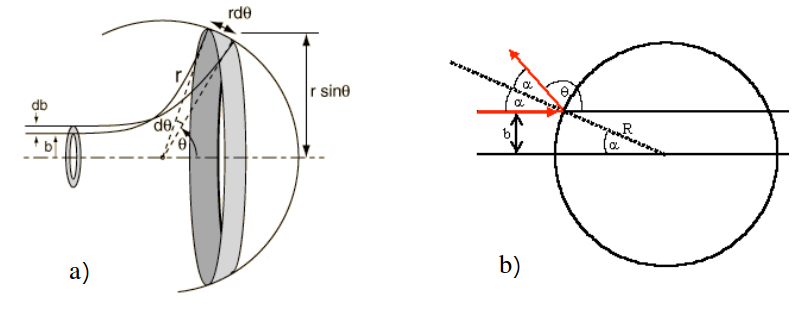
\includegraphics[width=0.9\textwidth]{subatom-03-geom.png}
\centering
\caption{Geometria zrážky.}
\label{sf3:fig:geom}
\end{figure}

Počet častíc rozptýlených za jednotku čase medzi ($\theta$, $\theta + d\theta$) je rovný počtu prichádzajúcich častíc za jednotku času medzi ($b$, $b+ db$), viď obrázok (\ref{sf3:fig:geom}, vľavo). Preto, pre dopadajúci tok $j_i$, počet častíc rozptýlených do uhlu $d\Omega=2\pi \sin\theta d\theta$ za jednotku času je daný
$$ Nd\Omega = 2\pi \sin\theta d\theta N = 2\pi b j_i db $$.

Definícia diferenciálneho účinného prierezu je nasledovná: podiel počtu častíc, ktoré sa rozptýlili do smeru ($\theta$,$\phi$) za jednotku času a dopadajúcim tokom častíc. Podľa tejto definície píšeme
$$ \frac{d\sigma(\theta)}{d\Omega} = \frac{N}{j_i} = \frac{b}{\sin\theta} \bigg\vert \frac{db}{d\theta} \bigg\vert. $$

Z obrázku (\ref{sf3:fig:geom}, vpravo) môžme ľahko nahliadnuť v akom vzťahu sú parameter $b$ a uhol $\theta$:
$$ b(\theta)=R\sin\alpha = R\sin\bigg(\frac{\pi - \theta}{2} \bigg)=-R\cos\bigg(\frac{\theta}{2} \bigg). $$
Potom dostaneme
$$ \bigg\vert \frac{db}{d\theta} \bigg\vert = \frac{R}{2}\sin\bigg(\frac{\theta}{2} \bigg) $$
Vložením všetkého do definície diferenciálneho účinného prierezu dostávame
$$ \frac{d\sigma(\theta)}{d\Omega} = \frac{R^2}{4} \hspace{1cm} \rightarrow \hspace{1cm} \sigma = \int \frac{d\sigma}{d\Omega}d\Omega=\pi R^2 $$
Dostávame presne taký istý výsledok ako sme povedali na začiatku, že prierez sa rovná projekcii plochy gule.

Rozptylový účinný prierez môže byť definovaný v jadrovej, atómovej a časticovej fyzike pre zrážky zrýchleného zväzku častíc jedného typu s pohyblivým alebo stacionárnymi terčom, ktorý je zložený z iného typu častíc. Pravdepodobnosť, že dôjde k akejkoľvek zrážke (reakcií) je úmerná práve účinnému prierezu danej reakcie. 

Predpokladajme, že na časticu \textbf{b} dopadá zväzok častíc typu \textbf{a}. Dochádza tým pádom k reakcií
$$ a+b \rightarrow c+d.$$
Experimentálne sa meria počet častíc jedného typu, ktoré prejdu za dobu $\Delta t$ plochou $\Delta S$.

Predpokladajme teda, že za jednú sekundu prejde elementom $\Delta S$ počet $\Delta N_2$ častíc typu \textbf{c}. Plošný element vymedzuje priestorový uhol $d\Omega$, pre ktorý platí
$$ d\Omega = \frac{dS}{R^2},$$ 
kde $R$ je vzdialenosť terčíka a plochy $\Delta S$, viď obrázok (\ref{sf3:fig:uhol}).

\begin{figure}[!h]
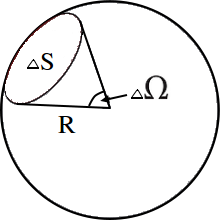
\includegraphics[width=0.3\textwidth]{subatom-03-uhol.png}
\centering
\caption{Priestorový uhol.}
\label{sf3:fig:uhol}
\end{figure}

Počet produkovaných častíc $\Delta N_2$ musí byť úmerný hustote toku častíc $n_1$ v dopadajúcom zväzku (pričom $[n_1]=m^{-2}s^{-1}$) a celkovému počtu ostreľovaných častíc v objeme $V$, ktorý sa dá vyjadriť pomocou hustoty častíc $n_2$ a plochy terča $S$ ako
$$ n_2V = n_2dS,$$
kde hrúbka $d$ sa predpokladá dosť malá nato, aby všetky častice terčíka mali voči zväzku rovnaké podmienky (priblíženie tenkého terčíka). Ďalej je počet vzniknutých častíc $\Delta N_2$ úmerný veľkosti priestorového uhla $d\Omega$ a pravdepodobnosti, že pri zrážke dôjde k produkcii častice \textbf{c}, ktorá vyletí do požadovaného uhla, tuto pravdepodobnosť značíme $\sigma(\theta, \varphi)$.

Pri voľbe osi-z v smere zväzku, môžme písať
$$ dN_2(\theta, \varphi) = n_1dn_2S \sigma(\theta, \varphi)d\Omega $$ 
$$ \frac{d\sigma}{d\Omega} \equiv \sigma(\theta, \varphi) = \frac{1}{n_1dn_2S}\frac{dN_2(\theta, \varphi)}{d\Omega}. $$
Veličina $d\sigma/d\Omega$ je vlastne diferenciálny účinný prierez. Keď preintegrujeme cez všetky možné uhly tak dostávame integrovaný účinný prierez, ktorý vyzerá vo všeobecnosti nasledovne
$$ \sigma = \int \frac{d\sigma}{d\Omega}d\Omega $$.

V teórii rozptylu sa taktiež definuje veličina, ktorá nejak súvisí z účinným prierezom. Táto veličina sa nazýva \textbf{luminozita} a je definovaná ako podiel počtu zrážok ($N$) detekovaných v určitej dobe a interakčného účinného prierezu ($\sigma$)
$$ L = \frac{1}{\sigma} \frac{dN}{dt}.$$
Táto veličina nezávisí na typu reakcie ale na vlastnostiach zväzku v urýchľovači ako napríklad šírka alebo rýchlosť zväzku a vlastnostiach terčíka ako napríklad jeho veľkosť a hustota. Luminozita ma rozmer $cm^{-2}s^{-1}$. Niekedy sa tiež zavádza tzv. integrovaná luminozita, čo je celková luminozita za určitý časový úsek a je daná vzťahom 
$$ I = \int L dt.$$

\textbf{Celkový účinný prierez} je daný 
$$ \sigma_{Total} = \sum_i \sigma_i,$$
kde $\sigma_i$ sú účinné prierezy všetkých procesov, ktoré môžu v látke nastáť (napríklad pružný a nepružný rozptyl, radiačný záchyt, štiepenie ... ). Celkový účinný prierez tak dáva pravdepodobnosť, že častica v látke bude interagovať nejakým procesom.

Celkový účinný prierez patrí k základným veličinám, ktoré je potrebné vedieť pre výpočet ďalších odvodených parameterov. Je možné ho spočítať tzv. transmisnou metódou. ktorá spočíva v zaznamenaní rozdielu v intenzitách častíc pred a za terčom. Používa sa nasledovný vzťah
$$ I = I_0e^{-N\sigma_{Total}}.$$
Z tohto vzťahu sme schopný spočítať daný účinný prierez ako
$$ \sigma_{Total} = \frac{1}{N}\ln \bigg( \frac{I_0}{I} \bigg),$$
kde $N$ počet častíc v terči v $cm^2$, $I$ je intenzita za terčom a $I_0$ intenzita pred terčom.

Ďalej definujeme \textbf{makroskopický účinný prierez} ako 
$$ \Sigma_i = N \sigma_i,$$
kde $N$ udáva počet častíc na jednotku objemu, $[N]=cm^{-3}$ a $\sigma_i$ je účinný prierez danej reakcie - často sa tento účinný prierez označuje ako mikroskopický účinný prierez. Rozdiel medzi makroskopickým ($\Sigma$) a mikroskopickým ($\sigma$) účinným prierezom je nasledovný: 
\begin{itemize}
\item mikroskopický účinný prierez ($\sigma$): reprezentuje efektívnu plochu jediného terčikového jadra pre dopadajúcu časticu $\sim cm^2$
\item makroskopický účinný prierez ($\Sigma$): reprezentuje efektívnu plochu všetkých terčikových jadier, ktoré sa nachádzajú v terčíku $\sim cm^{-1}$
\end{itemize}
 
Pomocou makroskopického účinného prierezu sme schopný zadefinovať pravdepodobnosť, že častica prejde v látke vzdialenosť $x$ bez akejkoľvek interakcie
$$ p(x) = e^{-\Sigma x}.$$
\begin{itemize}
\item $p(0) = 1$: to znamená, ze častice má 100$\%$ pravdepodobnosť, že na dráhe s dĺžkou 0 nebude interagovať 
\item $p(\infty) = 0$: to znamená, že častica ma 0$\%$ pravdepodobnosť, že na dráhe s nekonečnou dĺžkou nebude interagovať
\end{itemize}

Pomocou makroskopického účinného prierezu sme schopný zadefinovať ďalšiu užitočnú veličinu: \textbf{stredná voľná dráha ($\lambda$)}. Tá je definovaná ako priemerná vzdialenosť, ktorú častica prejde v materiály bez akejkoľvek interakcie, čo sa dá matematický vyjadriť nasledovne
$$ \lambda = \int x p(x) dx = x(e^{-\Sigma x}) (\Sigma dx)  = \frac{1}{\Sigma} = \frac{1}{N\sigma},$$
kde prvá zátvorka znamená, ze častice prejde vzdialenosť $x$ bez akejkoľvek interakcie, druhá zátvorka znamená, že častica podstúpi prvú interakciu v oblasti $dx$.

\subsection{Účinný prierez v kvantovej teórii poľa}
Základnou veličinou popisujúcou rozptylový proces 
$$ 1+2 \rightarrow 3+4+5+...+n $$
je diferenciálny účinný prierez v obecnom tvare
$$ d\sigma = \frac{ \overline{ \vert M_{fi}\vert^2 }}{4E_1E_2\vert \vec{v_1}-\vec{v_2} \vert} dLips_{n_f},$$
kde $M_{fi}$ označuje invariantnú amplitúda prechodu daného procesu. Ďalej Lorentzovský invariantný flux faktor je definovaný ako 
$$ \frac{1}{4E_1E_2\vert \vec{v_1} - \vec{v_2} \vert} = \frac{1} {4\sqrt{ (p_1p_2)^2 - m_2^2 m_2^2}}.$$
Lorentzovský invariantný je taktiež faktor fázového priestoru 
$$ dLips_{n_f} = (2\pi)^4\delta^{(4)} \bigg(p_1+p_2-\sum_{i=3}^{n_f}p_i \bigg)\prod_{i=3}^{n_f}\frac{d\vec{p_i}}{(2\pi)^32E_i},$$
kde $E_i$ je energia i-tej častice, ktorá sa pohybuje rýchlosťou $\vec{v}_i$.

\subsection{Typické hodnoty účinných prierezov}
Veľmi silná závislosť účinného prierezu na energii častíc ale aj druhu interakcie. Hodnoty sa pohybujú vo veľmi veľkom rozsahu:
\begin{itemize}
\item Silná interakcia - ($\sim 0.01\,barn$ - $\sim 10^4\,barn$) - (interakcie jadier a iných hadrónov)
\item Slabá interakcia - ($\sim 10^{-19}\,barn$) - (interakcie neutrín)
\item Elektromagnetická interakcia - ($\sim 0.1\,\mu barn$ - $\sim 10\,mbarn$) - (interakcie nabitých leptónov a fotónov)
\end{itemize} 


Medzi známe elektromagnetické účinné prierezy patri nepochybne Rutherfordov účinný prierez, ktorý spočíva na elektromagnetickej interakcii medzi dvomi nabitými časticami a ktorý ma tvar
$$ \frac{d\sigma}{d\Omega} = \frac{Z_1^2Z_2^2\alpha^2(\hbar c)^2}{16E^2\sin^4(\theta/2)}.$$
Ďalším elektromagnetickým procesom Thomsonov účinný prierez, ktorý je založený na elastickom rozptyle elektromagnetického žiarenia na voľnej nabitej častici, jeho tvar je nasledovný
$$ \sigma = \frac{8\pi}{3} \bigg(\frac{\alpha \hbar c}{mc^2} \bigg)^2.$$ 
Diferenciálny účinný prierez pre elektrón-mión rozptyl prostredníctvom fotónu má tvar
$$ \frac{d\sigma}{d\Omega} = \frac{e^4}{32\pi s}\frac{s^2+t^2}{u^2} $$
Posledný príklad na elektromagnetický účinný prierez si uvedieme pre proces ($e^+e^- \rightarrow \mu^+ \mu^-$) cez fotón
$$ \sigma = \frac{4 \pi \alpha^2}{3s^3} $$
Pre proces ($ e^+e^- \rightarrow q \bar{q} $) máme 
$$ \sigma = \frac{2\pi \alpha^2}{s^3} \sum_f Q^2_f \bigg[ 2m_f^2(m^2_f+2s)+\frac{2}{3}s^2 \bigg], $$
kde $Q_f$ a $m_f$ predstavuje náboj a hmotnosť kvarku s príchuťou f.
Medzi účinne prierezy slabých interakcii môžme zaradiť prierez pre rozptyl neutrína na kvarku
$$ \frac{d\sigma(\nu+q)}{dy} = \frac{d\sigma(\bar{\nu}+\bar{q})}{dy} = \frac{G_F^2s}{\pi} $$
alebo pre interakciu kvarku a antineutrína
$$ \frac{d\sigma(\nu+\bar{q})}{dy} = \frac{d\sigma(\bar{\nu}+q)}{dy} = \frac{G_F^2s}{\pi}(1-y)^2 $$
Použitím týchto účinných prierezov môžme napísať prierez pre interakciu neutrína, antineutrína s nukleónom
$$\sigma(\nu N )=\frac{G_F^2s}{2\pi} \bigg[f_g+\frac{1}{3}f_{\bar{g}} \bigg] \hspace{1cm} \sigma(\bar{\nu} N )=\frac{G_F^2s}{2\pi} \bigg[\frac{1}{3}f_g+f_{\bar{g}} \bigg] $$
kde $f_g=0.41$ a $f_{\bar{g}}=0.08$.
\subsection{Interakcie žiarenia s hmotou} 
Energetické straty častíc pri prechode hmotou, procesy interakcie nabitých častíc a fotónou, aplikácie. Túto časť nebudeme veľmi rozpisovať, keďže ju mame podrobne spísanú v sekcii Jadrová spektroskopia. Spomenieme len nejaké veci a nejaké aplikácie.
\newline

Termín žiarenie sa vzťahuje na emisiu a šírenie energie cez priestor alebo materiál. Máme dva typy žiarenie
\begin{itemize}
\item elektromagnetické žiarenie
\item časticové žiarenie
\end{itemize}

Elektromagnetické žiarenie sa šíri prostredníctvom svetelných, tepelných vĺn, gama alebo röntgenového žiarenie. Tieto dva typy žiarenia majú široké uplatnenia: veda, medicína, priemysel .... 

Časticové žiarenie sa vzťahuje na energiu propagovanú cestujúcimi časticami, ktoré majú v každom okamihu určitú pokojovú hmotnosť, hybnosť. Poznáme elektrónové, protónové, neutrónové žiarenie ale aj iné.

Pri prechode röntgenového lúča alebo gama lúča prostredím, vznikajú interakcie medzi fotónom a hmotou a tým dochádza k prenášaniu energie z lúčov do média. Počiatočný krok prenosu energie zahŕňa uvoľnenie elektrónov z atómov absorpčného média, ktoré zase prenášajú svoju energiu tým, že produkujú ionizáciu a excitáciu atómov pozdĺž ich dráhy. Fotónový lúč môže podstúpiť nasledujúce procesy
\begin{itemize}
\item Útlm sa vzťahuje na zoslabenie žiarenia. Môže nastať v dôsledku rozptylu alebo absorpcie.
\item Absorpcia sa vzťahuje na predanie energie z lúča do ožarovaného materiálu.
\item Rozptyl sa vzťahuje na zmenu smeru fotónov a prispieva tak k útlmu a absorpcii.
\item Transmisia fotónu nastáva, keď ktorýkoľvek fotón nepodstúpi vyššie uvedené procesy. Vtedy fotón proste prejde cez materiál.
\end{itemize}

Existuje päť hlavných fyzikálnych procesov, ktoré sú zodpovedné za zoslabenie fotónového lúča: Koherentný rozptyl, Fotoelektrický efekt, Comptonov efekt, Tvorba párov, Foto rozpad.

Koherentný rozptyl, tiež známy ako elastický rozptyl zahŕňa napríklad Thomsonov rozptyl, Rutherfordov rozptyl, Rayleigh rozptyl atď. Je to jeden z procesov, ktoré možno ľahšie opísať vlnami ako fotónmi. Okrem toho je to aj jedna z interakcií, kde sú zapojené viazané elektróny. Röntgenové lúče prechádzajúce v blízkosti atómu a spôsobujú, že viazané elektróny budú vibrovať takou istou frekvenciou akú majú dané röntgenové lúče. Tieto elektróny následne vyžarujú žiarenie rovnakej frekvencie do všetkých smerov.
Avšak, žiadna energia nie je absorbovaná. Je to forma útlmu bez absorpcie. Táto interakcia má malú dôležitosť v praktickej rádioterapii, ale je dôležitá v röntgenovej kryštalografii. Keďže táto interakcia zahŕňa viazané elektróny, vyskytuje sa viac v materiáloch s vyšším atómovým číslom a tiež viac s nízkymi energetickými vyžarovaniami.

Pri fotoelektrickom efekte sa fotón úplne pohltí po interakcii s viazaným elektrónom, pričom časť energie tohto fotónu sa použije na odtrhnutie elektrónu z atómového plášťa a zvyšok sa prenesie do kinetickej energie elektrónu. Ionizovaný atóm získava elektrickú neutralitu preskupením ostatných orbitálnych elektrónov. Elektróny, ktoré prechádzajú týmto prerozdelením, odovzdajú časť energie vo forme fotónu známeho ako charakteristické žiarenie atómu. Absorpcia tohto charakteristického žiarenia vo vnútri atómu môže viesť k emisii Augerových elektrónov. Tieto elektróny majú monoenergetický charakter. Uhlová distribúcia elektrónov emitovaných vo fotoelektrickom procese závisí od fotónovej energie. Zo zvyšovaním fotónovej energie sa fotónové elektróny emitujú v doprednejšom smere. Ako ukazuje graf na obrázku (\ref{sf3:fig:photo}), existujú diskontinuity v útlme pri špecifických fotónových energiách. Tieto diskontinuity sa nazývajú absorpčné hrany. Tieto absorpčné hrany zodpovedajú väzbovým energiám elektrónov v
rôznych vrstvách.

\begin{figure}[!h]
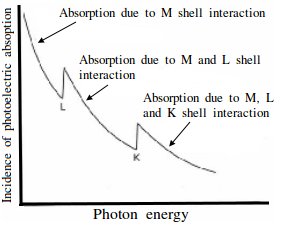
\includegraphics[width=0.5\textwidth]{subatom-03-fotoefekt.png}
\centering
\caption{Útlm fotonového lúča vo fotoelektrickom jave.}
\label{sf3:fig:photo}
\end{figure}

Fotoelektrický efekt má niekoľko dôležitých dôsledkov pre praktickú rádiológiu:
\begin{itemize}
\item V diagnostickej rádiológii je primárny režim interakcie fotoelektrický.
\item V terapeutickej rádiológii spôsobujú nízkoenergetické lúče nadmernú absorpciu energie v kostiach.
\end{itemize}

Fenomén absorpčných okrajov je dôležitý z dvoch rôznych dôvodov:
\begin{itemize}
\item Na týchto absorpčných hranách sú fotóny s nízkou energiou menej oslabené, a preto sú prenikavejšie ako fotóny s vysokou energiou.
\item Látka je relatívne priehľadná svojmu vlastnému charakteristickému žiareniu.
\end{itemize}

Comptonov efekt, tiež známy ako nekoherentný rozptyl. V tejto interakcii fotón interaguje s voľným elektrónom. 
Keď fotón interaguje s elektrónom odovzdá časť svojej energie elektrónu. Uhol rozptylu fotónu, energia elektrónu a energetická strata fotónu sú navzájom previazané. Z formuly pre Comptonov rozptyl vieme, že zmena vlnovej dĺžky nie je závislá ani na ožarovanom materiáli ani na energii žiarenia, ale len na uhle, cez ktorý je žiarenie rozptýlené. Tento efekt spôsobuje aj útlm aj absorpciu. K párovej produkcii nič nové nepridáme. 

Foto nukleárna reakcia nastáva, keď fotón má energiu väčšiu ako väzobná energia samotného jadra. V tomto prípade fotón vstupuje do jadra a emituje z neho časticu. Fotón sa úplne pohltí a akákoľvek zvyšná energia sa stáva kinetickou energiou emitovanej častice. Táto metóda sa taktiež využíva v medicíne.

Časticové žiarenie sa dá rozdeliť do dvoch kategórii - nabite a nenabité časticové žiarenie. Nabité častice, ktoré sa najviac využívajú v rádioterapii sú elektrón, protón a pión.

Poznáme dva spôsoby ako elektrón interaguje a odovzdáva energiu hmote - ionizácia a excitácia (viacej dôležité v materiáloch s menším atómovým číslom), brzdné žiarenie (viacej dôležitejšie v materiáloch s väčším atómovým číslom). Ionizácia vedie k odobratiu elektrónu z atómu. Ak tieto uvoľnené elektróny majú dostatočne veľkú energiu môžu spôsobovať taktiež ionizáciu - $\delta$ elektróny. Elektróny sú ľahké častice so zanedbateľnou hmotnosťou a jedným záporným nábojom. Výsledkom je, že prenikajú hlbšie než iné nabité častice, ale súčasne podliehajú väčšiemu rozptylu.

Protony a $\pi$ mezóny sú nabité častice, ktoré vykazujú javy Braggovho píku, to znamená zvýšenej ionizácie vyskytujúcej sa tesne pred zastavením častice v látke. Tento fenomén sa využíva pri liečbe rakoviny. Avšak problém je, že generovanie týchto nabitých častíc je dosť náročné pretože sa nato vyžadujú drahé a veľké prístroje.

Neutrónové žiarenie je nepriamo ionizujúce nenabité žiarenie, ktoré interaguje s jadrom dvoma spôsobmi: recoilom protónov z jadier, jadrovým rozpadom. Najúčinnejší recoil je viditeľný vo vodíkovom jadre, čo vedie k maximálnej absorpcii. To je výhoda, pretože väčšina mäkkých tkanív v tele obsahuje veľkú časť vodíka. Tento jav má niektoré praktické dôsledky:
\begin{itemize}
\item Hydrogénne materiály, ako napríklad tuky, absorbujú neutrony viac než ťažšie materiály, a preto je o 20$\%$ vyššia absorpcia v tuku v porovnaní so svalmi.
\item Nižšie atómové materiály (napríklad tuky a parafín) sú lepšie v prípade neutrónového tienenia v porovnaní s olovom, pretože dochádza k väčšej absorpcii.
\end{itemize}
Recoil protóny, ktoré sa aktivovali po interakcii s neutrónmi sú ďalšou príčinou ionizácie. Neutróny, ktoré sú nenabitými časticami, prenikajú hlboko do hmoty. Napriek týmto atraktívnym rádiobiologickým a fyzikálnym vlastnostiam sa neutróny bežne nepoužívajú pri praktickej rádioterapii kvôli technickým ťažkostiam pri výrobe týchto lúčov, ako aj kvôli ich komplikovanej dozimetrii. Na obrázku (\ref{sf3:fig:dose}) môžme vidieť rozlične dávky časticového žiarenia vo vode.

\begin{figure}[!h]
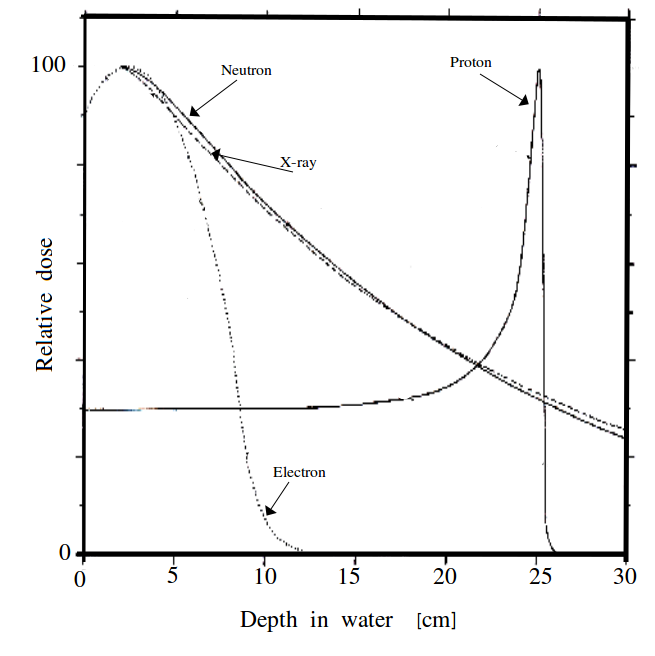
\includegraphics[width=0.8\textwidth]{subatom-03-dose.png}
\centering
\caption{Relatívne dávky rôznych druhov žiarenia.}
\label{sf3:fig:dose}
\end{figure}

\subsection{Protónová terapia a Braggov pík}
Röntgenová a protónová terapia sú techniky rádioterapie používané v medicíne. Röntgenová terapia používa fotóny na ožarovanie chorých tkanív, zatiaľ čo protónová terapia používa lúče energetických protónov, ktoré majú veľmi odlišné fyzikálne vlastnosti ako fotóny.

Predtým ako tieto žiarenia dosiahnú nádor, musia prejsť cez pokožku a okolité tkanivo pacienta. Fotón, ktorý nemá ani hmotnosť ani náboj, je vysoko penetrujúci. Popri tomu ako tento fotón prechádza tkanivom odovzdáva energiu okolitému tkanivu. Avšak, najväčšie množstvo energie tohto žiarenia sa odovzdá tkanivu nachádzajúce sa v hĺbke $0.5-3\,cm$ od pokožky pacienta. Potom odovzdaná dávka tohto žiarenia postupne klesá a v mieste kde sa nachádza nádor bude dávka tohto žiarenia oveľa menšia. Navyše, keďže fotóny nie sú zastavené ľudským tkanivom, opúšťajú telo pacienta (výstupná dávka).

Naopak, protón je ťažká a nabitá častica, ktorá postupne stráca svoju rýchlosť, pretože interaguje s ľudským tkanivom. Je ľahko ovládateľný a dodáva maximálnu dávku v presnej hĺbke, ktorá je určená množstvom energie, ktorú cyklotrón (prostredníctvom urýchľovača) dodal tomuto protónu. Tento protón môže dosahovať hĺbku až 32 cm. Protón je veľmi rýchly, keď vstupuje do tela pacienta a ukladá len malú dávku na jeho ceste. Absorbovaná dávka sa zvyšuje veľmi postupne s vyššou hĺbkou a nižšou rýchlosťou protónu. Tesne pred zastavením, protón odovzdá maximálnu dávku okolitému tkanivu. Tento efekt je známy ako Braggov pík. Chovanie protónu sa dá presne určiť a lúč môže byť nasmerovaný tak, aby Braggov pík nastával presne v mieste nádoru. Ihneď po tomto výbuchu energie sa protón úplne zastaví. Protónová terapia preto umožňuje cielené ožarovanie nádorov vo vnútri tela. Týmto sme schopný ušetriť zdravé bunky pacienta a ponúknuť tak oveľa menej invazívnu liečbu rakoviny.

Braggov pík: keď rýchlo nabitá častica prechádza hmotou, ionizuje atómy materiálu a ukladá dávku pozdĺž cesty. K piku dochádza, pretože interakčný účinný prierez sa zvyšuje, keď sa energia nabitých častíc znižuje. Množstvo energie, ktorú častica odovzdáva materiálu je nepriamo úmerná štvorcu rýchlosti tejto častice, čo vysvetľuje vrchol vyskytujúci sa tesne predtým, ako častica zastaví.

\subsection{Pozitrónová emisná tomografia}
Princípom metódy je lokalizácia miesta vzniku fotónov, ktoré v tele vznikajú pri anihilácii pozitrónov uvoľnených podanou rádioaktívnou látkou (rádiofarmakom) a elektrónov. Detekcia uvoľnených fotónov je usporiadaná tak, že je možná trojrozmerná rekonštrukcia aktivity rádiofarmaka v tele. 

Pacientovi sa pred vyšetrením podá rádiofarmakum s veľmi krátkym polčasom rozpadu. U PET sa využívajú rádiofarmaka, ktoré pri svojom rozpade produkujú pozitróny. Pozitrón po svojom vzniku anihiluje s elektrónom. K anihilácii dochádza rádovo v nanosekundách, behom ktorých sa vzniknutý pozitrón stihne presunúť od miesta vzniku len o niekoľko milimetrov. Pozitrón a elektrón zanikajú a z miesta anihilácie odlietajú v priamom uhle dva fotóny, každý s energiou $511\,keV$. Detektory sú umiestnené na prstenci okolo pacienta a detekujú takto vzniknuté fotóny. Detektory sú v tzv. koincidenčnom zapojení. To znamená, že  je zaznamenaný len súčasný záchyt dvoch, proti sebe idúcich fotónov vyletujúcich z tela pacienta. Toto opatrenie na jednej strane znižuje šum a na strane druhej, umožňuje viesť rovinou detekčného prstenca priamku, na ktorej došlo k rozpadu rádiofarmaka. Z veľkého množstva príkladov takýchto priamok možno zrekonštruovať aktivitu v jednotlivých bodoch roviny prechádzajúcej detekčným prstencom, teda získať tomografický rez telom pacienta. Princíp PET je načrtnutý na obrázku (\ref{sf3:fig:pet}).

Ako rádionuklid sa najčastejšie využívá: uhlík-11 (polčas rozpadu ~20 min), dusík-13 (polčas rozpadu ~10 min), kyslík-15 (polčas rozpadu ~2 min), a fluor-18 (polčas rozpadu ~110 min).

\begin{figure}[!h]
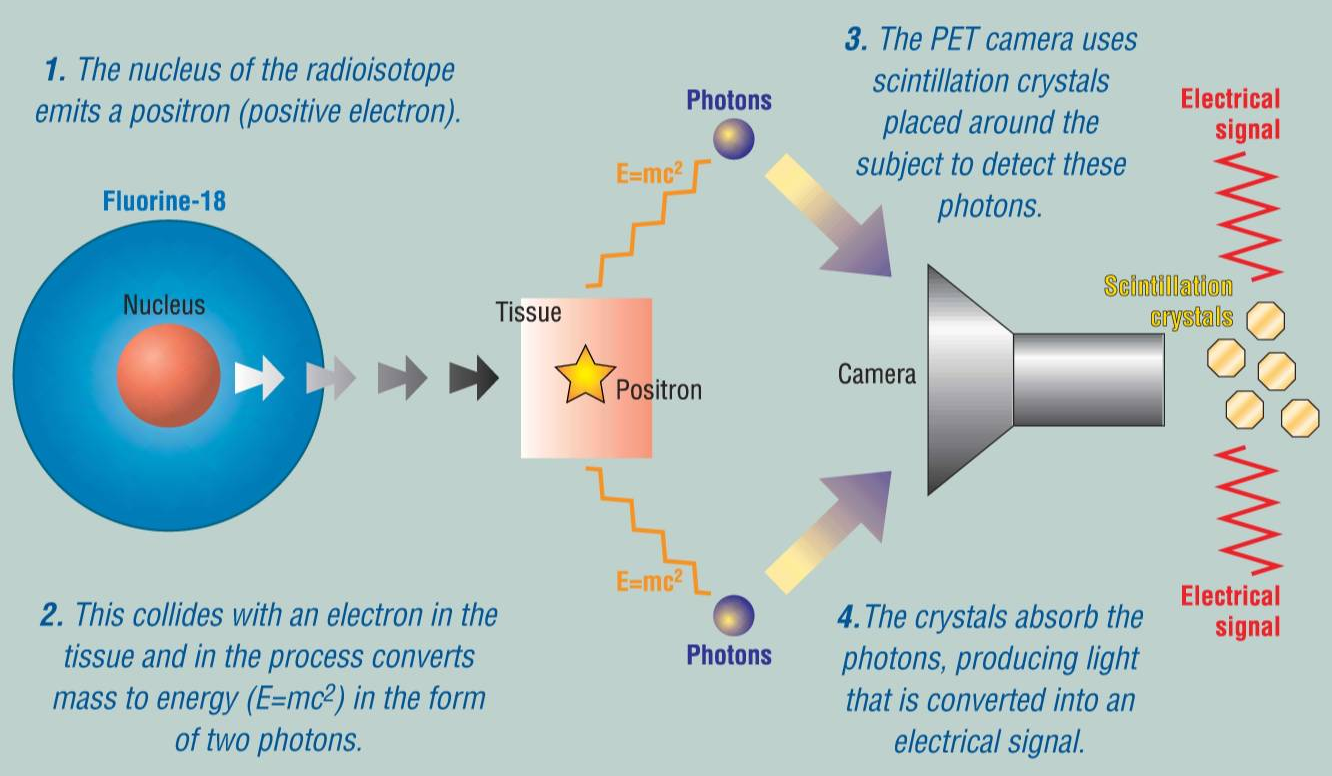
\includegraphics[width=0.65\textwidth]{subatom-03-PET.png}
\centering
\caption{Princíp fungovania PET.}
\label{sf3:fig:pet}
\end{figure}











\end{document}